\subsection{Fórum}
O desenvolvimento da página do fórum trouxe diversas dificuldades, entre elas, a gestão de filtros, pesquisas, a mostragem de tópicos e atualização dos mesmos.

\vspace{10mm}
\begin{figure}[htb]%
 \centering
 \subfloat[\centering Página de forum]{{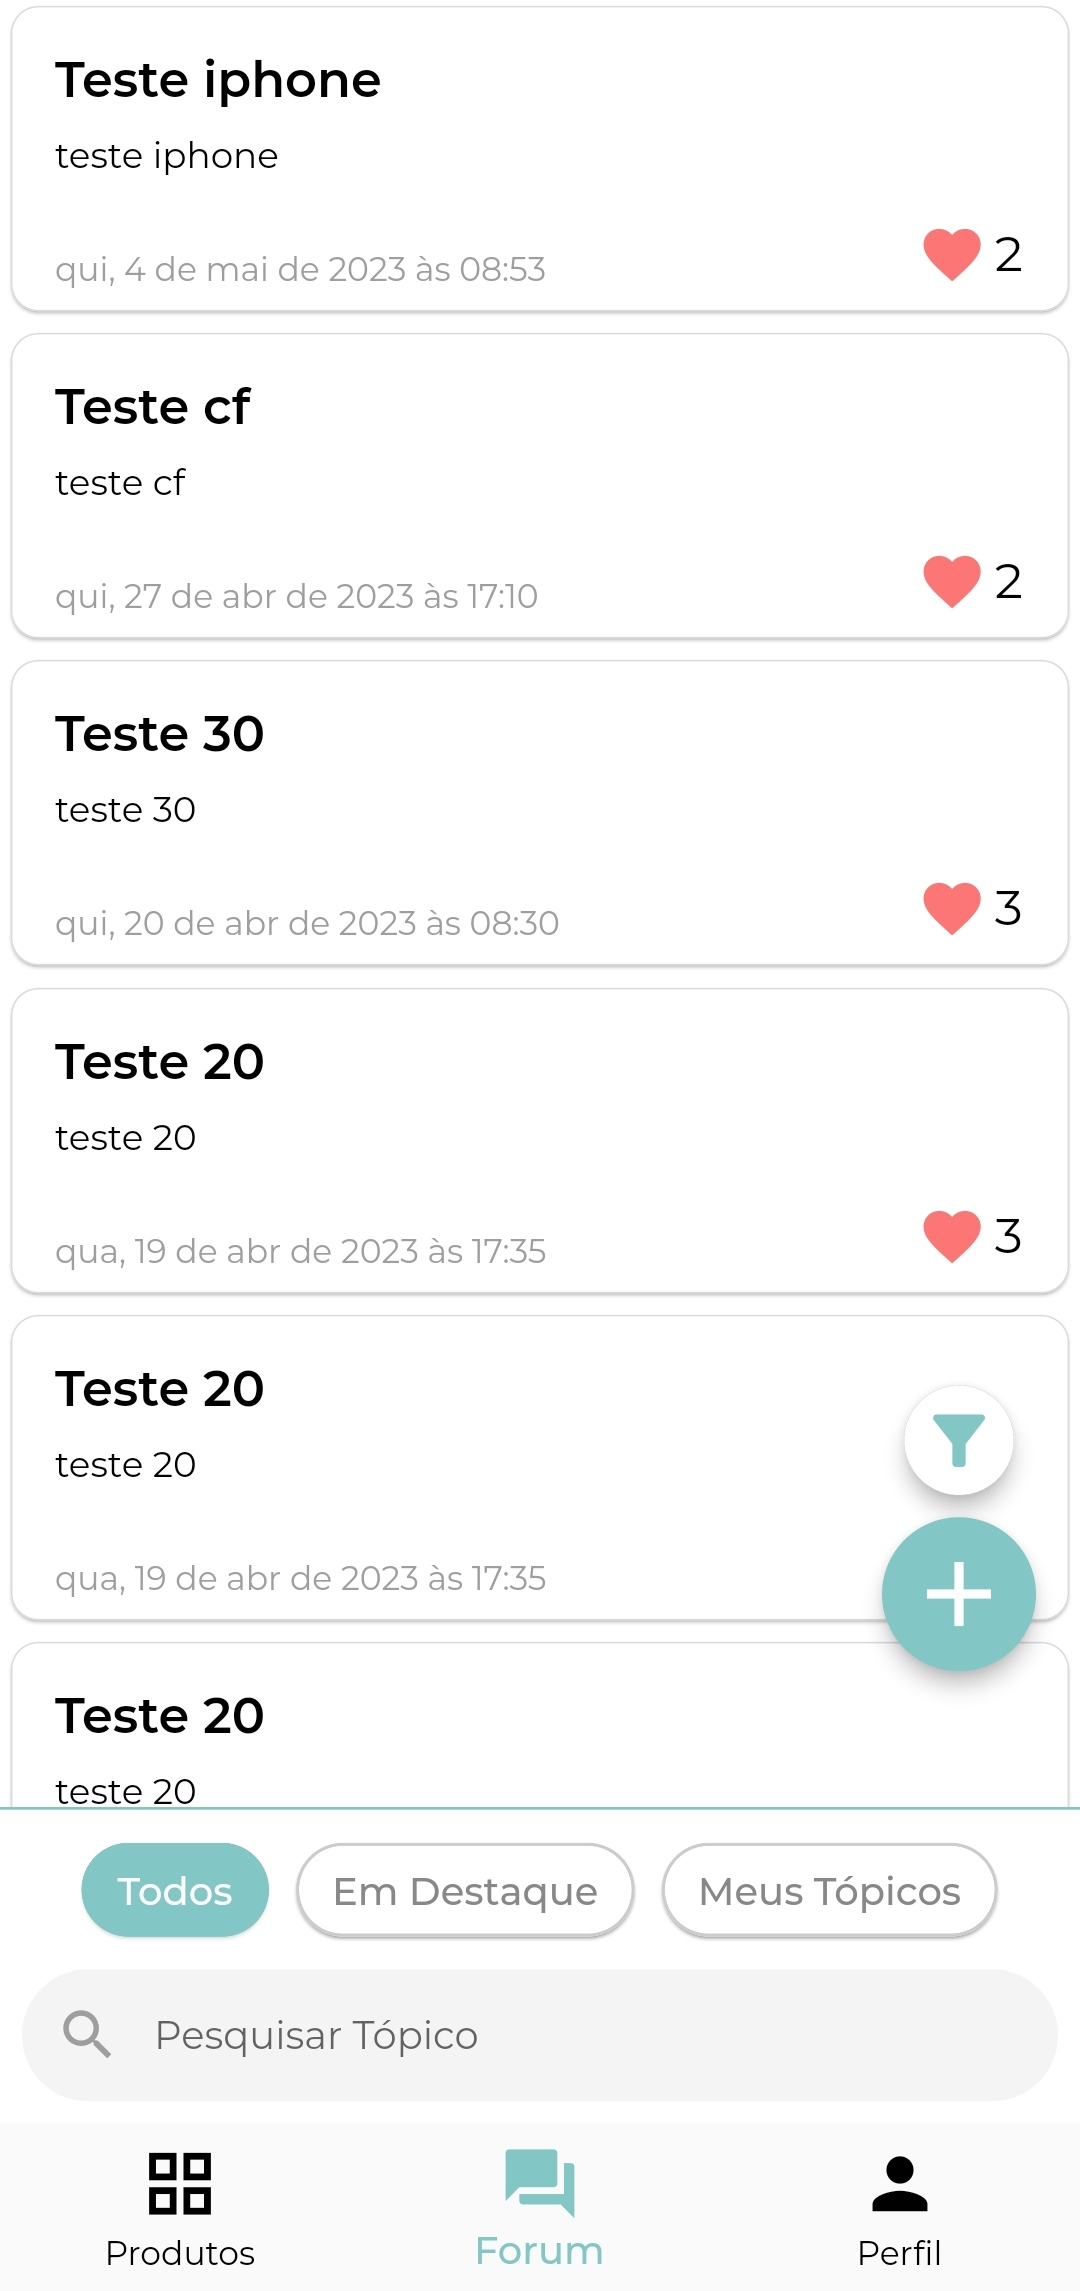
\includegraphics[width=0.3\textwidth]{images/implementacao/frontend/forum/1686055611203.jpg} }}%
 \qquad
 \subfloat[\centering Filtragem de tipo]{{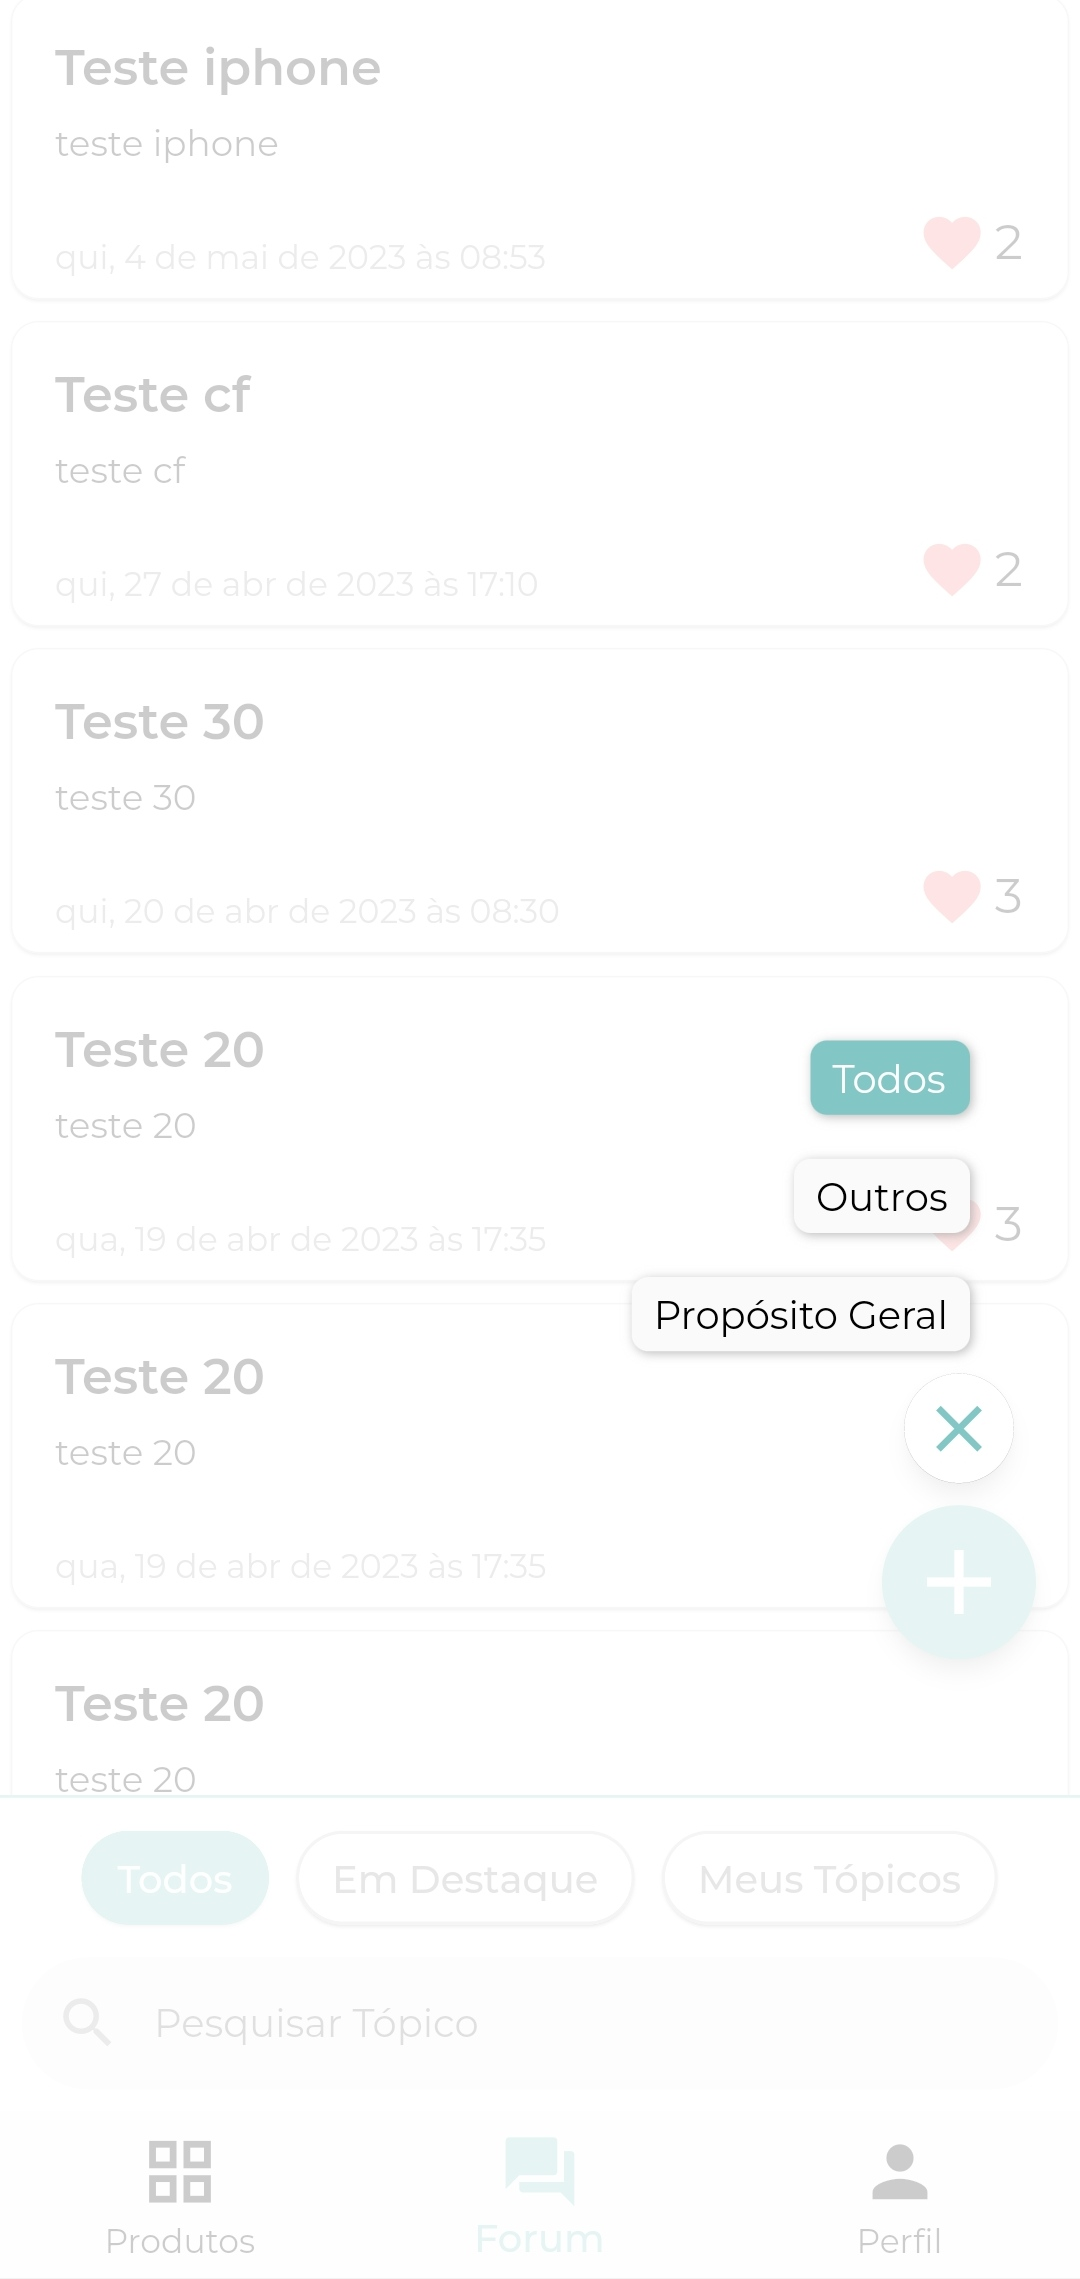
\includegraphics[width=0.3\textwidth]{images/implementacao/frontend/forum/1686055611213.jpg} }}%
 \label{fig:72}%
\end{figure}
\vspace{10mm}

\newpage

\subsubsection{Filtragem de tópicos}
O grande problema com a filtragem dos tópicos é que existem 3 tipos de filtros, o de categoria de tópico, o de tipo de tópico e o de pesquisa. 

Se algum filtro for alterado, os seguintes deverão ser novamente executados para garantir que todos permanecem aplicados. Inicialmente, este tipo de filtragem não era realizado, o que levava a diversos problemas, tais como, na realização de uma pesquisa, esta não era efetuada sobre os tópicos filtradas, o que levava a que a pesquisa fosse efetuada por todos os tópicos.

Outro problema detetado foi a troca de categorias, que por vezes, os filtros adicionavam-se, o que levava a que estes não apresentassem tópicos.

Sendo assim, foram criados métodos para auxílio na filtragem, tais como, uma prioridade, onde cada método invoca o método seguinte de forma encadeada. Primeiramente aplica-se o filtro de categoria, de seguida este envia o resultado para o método de filtragem por tipo e por fim, se existir algum tipo de pesquisa, os tópicos provenientes do método anterior serão filtrados.

\begin{figure}[htb]
 \centering
 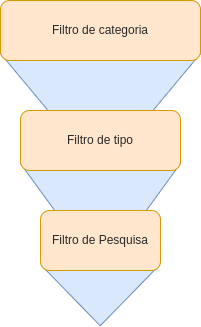
\includegraphics[width=0.25\textwidth]{images/implementacao/frontend/forum/filtros/filtros.png}
 \caption{Filtragem do forum}
 \label{fig:73}
\end{figure}

\newpage

\subsubsection{Carregamento de tópicos}
Inicialmente o carregamento de tópicos fazia-se por inteiro, desde carregamento de todos os tópicos, até todos os dados dos mesmos, visto que, não existiam muitos tópicos este não seria um problema para a \textit{\acrshort{api}}, mas, conforme os testes foram realizados a quantidade de tópicos existentes foi gradualmente aumentando, pelo que, foi possível visualizar o tempo de demora da resposta do servidor a aumentar, assim como, o desempenho da aplicação no fórum a piorar.

A resolução deste problema proveio com uma técnica de \textit{sliding window}, na qual os tópicos mantêm-se carregados, sendo que, a própria \textit{framework} consegue através da lista retirar de renderização os tópicos que o utilizador não consegue ver. 

Esta solução foi implementada através da utilização de três valores, quantidade de tópicos a obter, índice inicial e data do primeiro tópico. O valor de quantidade de tópicos a obter, inicialmente dez, permite limitar a quantidade de tópicos que a \textit{\acrshort{api}} irá processar, o que reduz o tempo de resposta. O índice inicial, indica qual o índice do primeiro elemento que se deseja obter da lista. A data do primeiro tópico, mantém uma referência temporal para obter tópicos, o que garante que a lista que está ser a visualizada é sempre a mesma.

Encontra-se no documento de anexos, no anexo 27, uma versão mais detalhada da Figura~\ref*{fig:74}.

\begin{figure}[htb]
 \centering
 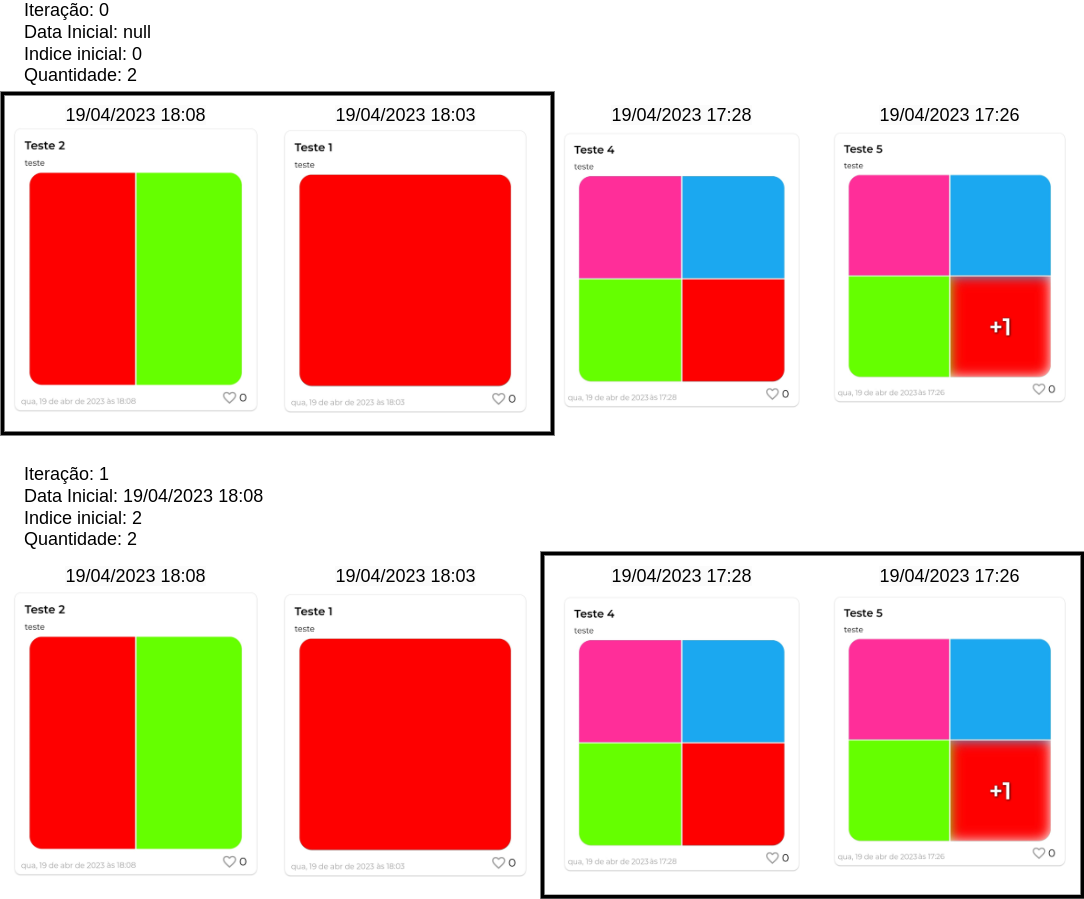
\includegraphics[width=0.75\textwidth]{images/implementacao/frontend/forum/loading_topics/topics_loading.png}
 \caption{Carregamento de tópicos}
 \label{fig:74}
\end{figure}
Também foi reduzida a quantidade de dados carregados por cada tópico, pelo que, apenas os comentários diretos ao tópico são carregados e não as respostas a estes, o que contribuiu para a melhoria do desempenho.

Por fim, sempre que o utilizador alcança o fim da lista de tópicos este poderá deslizar para carregar mais tópicos.

\newpage

\subsubsection{Detalhes de tópico}

A página de detalhes de tópico sofreu os mesmos problemas que a página anterior, o que levou à necessidade de aplicar a mesma solução sobre os comentários de tópico e sobre as respostas aos mesmos. Sendo assim são carregados os primeiros dez comentários e por fim, demonstrado ao utilizador quantos mais existem que poderá carregar, sendo carregados dez de cada vez.

Estes comentários podem conter respostas, sendo que estas conseguem ser carregadas também dez de cada vez e o utilizador consegue esconder ou mostrar estas.

Outro problema que surgiu no desenvolvimento da página de detalhes de tópico foi o destaque de um comentário. Este foi uma grande dificuldade, pois, com a nova implementação as mensagens não estão carregadas no momento do destaque da mensagem, pelo que, é necessário procurar a mesma nos comentários carregados, o que expande as respostas do comentário que contêm a reposta a destacar.

O destacamento das mensagens também continha um erro. Sempre que algo no ecrã é atualizado, este recarregava a animação de destaque, como solução este código foi movido para apenas ser executado no momento de inicialização do ecrã após todos os elementos se encontrarem devidamente carregados.

\begin{figure}[htb]
 \centering
 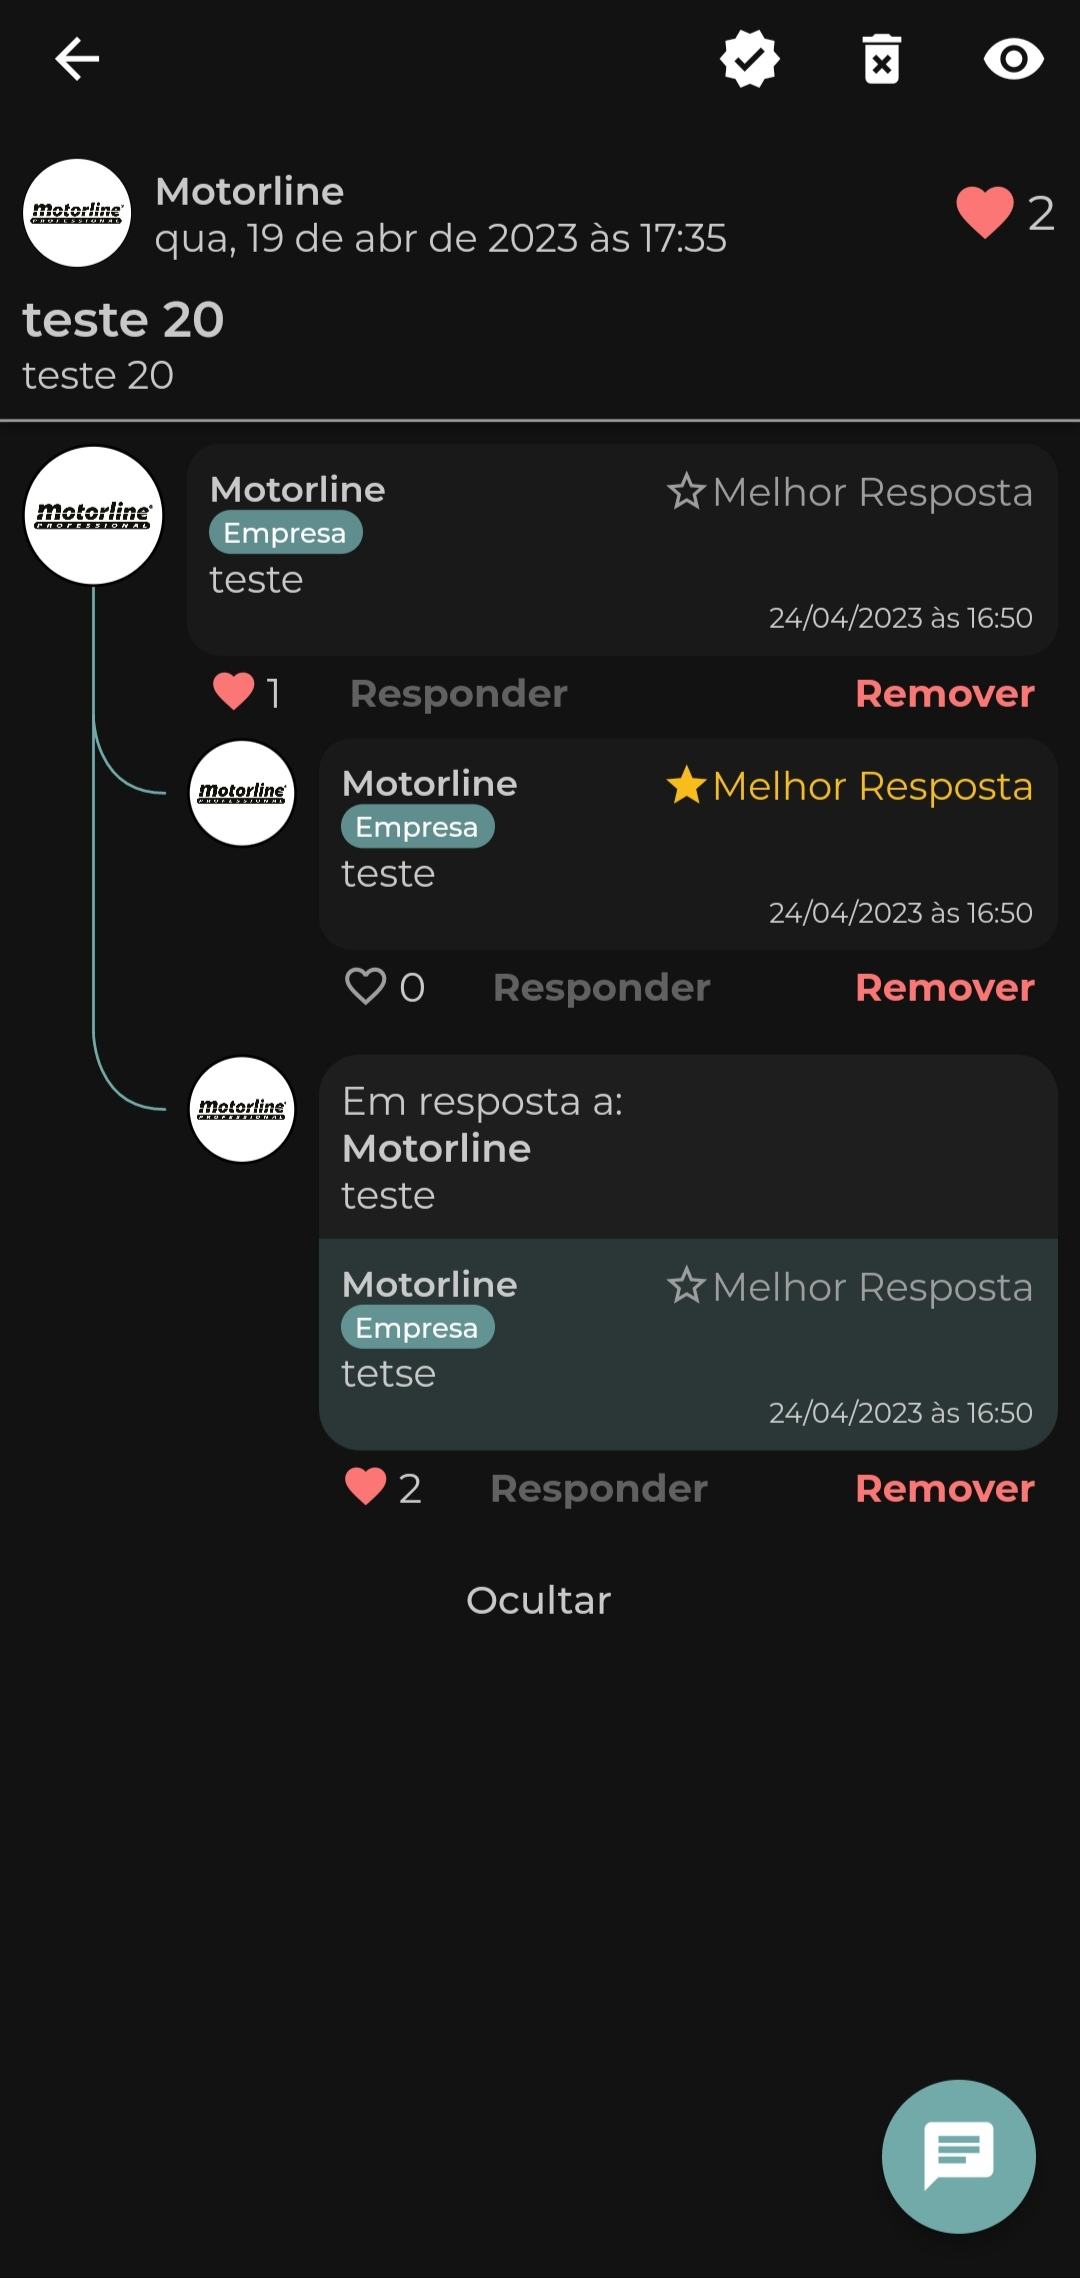
\includegraphics[width=0.35\textwidth]{images/implementacao/frontend/forum/loading_topics/1686062701127.jpg}
 \caption{Destaque de mensagens}
 \label{fig:75}
\end{figure}